\documentclass{beamer}

\usepackage[utf8x]{inputenc}
\usepackage{default}
\usetheme{Warsaw}
\usepackage{beamerthemesplit}
\usecolortheme{rose}%Light definition headings
\usefonttheme[onlysmall]{structurebold}
\setbeamerfont{title}{shape=\itshape,family=\sffamily}
%\setbeamercolor{background canvas}{bg=red!20}
%\usefonttheme[onlylarge]{structuresmallcapsserif}%Large headings
%\setbeamercolor{title}{fg=red!80!black,bg=red!20!white}
%\mode<handout>{\beamertemplatesolidbackgroundcolor{black!5}}
\usepackage{pdfpages}
\usepackage{textcomp}
\usepackage{amsmath}
\usepackage{geometry}
%\usepackage{subfig}
\usepackage{float}
\usepackage{graphicx}
%\floatstyle{boxed}
%\restylefloat{figure}
\title{\texttt{EduAerospace}}
\subtitle{AE 663 : Software Development Techniques for Engineering and Scientists}
%\author{Thammisetty Devakumar - 08001021 \\ Mustafa Mutiur Rahaman - 08D01022 \\ Shiv Kailash V - 08001022}
\date{\empty}


\begin{document}

\begin{frame}[label = Titlepage]
	\titlepage
	\vspace*{-3cm}
	\begin{figure}
		\centering
		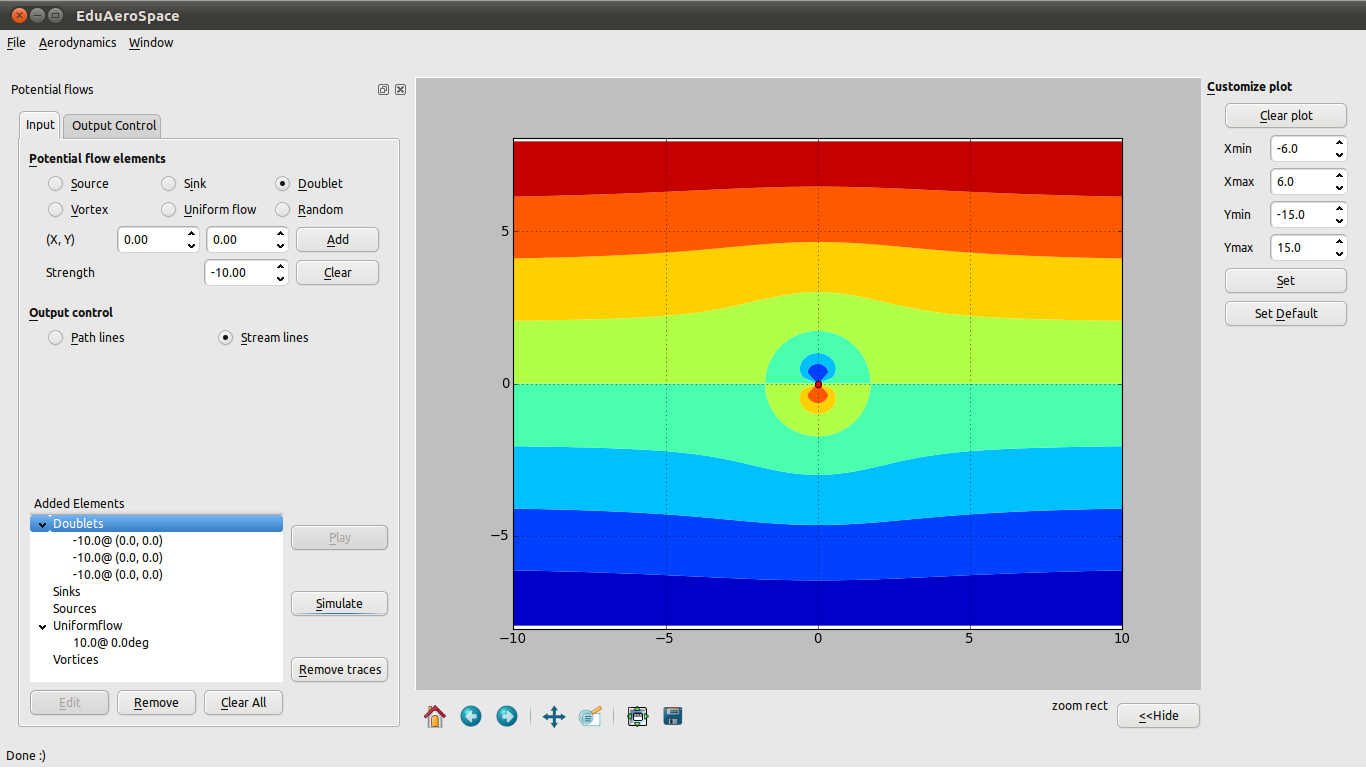
\includegraphics[width=0.8\textwidth]{Images/pic2.png}
	\end{figure}
\end{frame}

\section{Outline}
\begin{frame}[label = toc]
	\tableofcontents[pausesections]
\end{frame}
\section{CFD-1D}
\subsection{Advection}
\begin{frame}
	    \begin{itemize}
\item Implemented Advection Scheme
\begin{equation}
            u_t + c u_x = 0
\end{equation}
	     \begin{itemize}
\item Incorporated Schemes: FTFS,FTBS,FTCS,Upwind Scheme,LaxWendroff Scheme
\item FTBS
\begin{equation*}
            u^{n+1}_i = u^n_i - (c \frac{ \Delta t}{ \Delta x} ) * (u^n_i - u^n_{i-1});
\end{equation*}
\item LaxWendroff Scheme  $\lambda = c  \frac{\Delta t}{ \Delta x} $
\begin{equation*}	    
            u^{n+1}_i = u^n_i - ( ( \lambda / 2.0 ) (u^n_{i+1} - u^n_{i-1})) + ( ( \lambda^2 / 2.0)  (u^n_{i+1} 
- 2.0  u^n_i + u^n_{i-1}) )
\end{equation*}

	  \end{itemize}
% \end{itemize}
% 
% \end{frame}
% \begin{frame}
% \begin{itemize}  

\item Boundary Condition Incorporated
\begin{itemize}  
\item Free: Ghost Cell values equal to neighbour cell
\item Reflect: Ghost Cell velocity is opposite to neighbouring cell
\item Complement: Ghost Cell value equals to neighbour cell of other Ghost Cell
 \end{itemize}  
\end{itemize}  
\end{frame}

\subsection{Burger}
\begin{frame}
\begin{itemize}
 \item Implemented Burger Scheme

\begin{equation}
            u_t + u u_x = 0
\end{equation}
\item Initial Conditions
\begin{itemize}	  
\item backward step: For shock propagation and smearing
\item forward step: For expansion evolution and smearing
\item backward ramp: For shock formation from just a smooth slope
\item forward ramp: For expansion evolution from constant slope
\end{itemize}  
\item Scheme
\begin{itemize}	  
\item Lax Method
$u^{n+1}_i = \frac{(u^n_{i+1}+u^n_{i-1})}{2.0} - (\frac{\Delta t}{ \Delta x})\frac{( {u^n_{i+1}}^2- {u^n_{i-1}}^2) }{4.0} $
	    \end{itemize}
\end{itemize}  
\end{frame}
\subsection{ShockTube}
\begin{frame}
\begin{itemize}
 \item Implemented 1D Shock Tube Problem
\begin{itemize}	  
\item Implemented HLL,HLLC,Vanleer, Steger Warming, AUSM, $AUSM^+$,$AUSM^+up$
\item Incorported the various parameters for  $AUSM^+$,$AUSM^+up$
\item Incorported the various other parameters in Sod Shock Tube
\item Incorporated the Iteration Time step
\item Incorporated the option for various output paramters
\end{itemize}  
\end{itemize}  
\end{frame}


\subsection{Special Feartures}
\begin{frame}
\begin{itemize}
\item	Implemented tests.py, to check the user defined scheme.
\item	Incorporated runtime messages in Status Bar
\item	Incorporated user defined iterating time step
\item	Plot parameters can be changed while simulating
\item	Incorporated short keys for special buttons
\item	Incorporated value range for different parameters including decimal points.
\item	Incorporated mouse increment with parameter type
\end{itemize}

\end{frame}

%\begin{frame}
%	\begin{figure}
%		\centering
%		\subfloat[Uniform Flow]{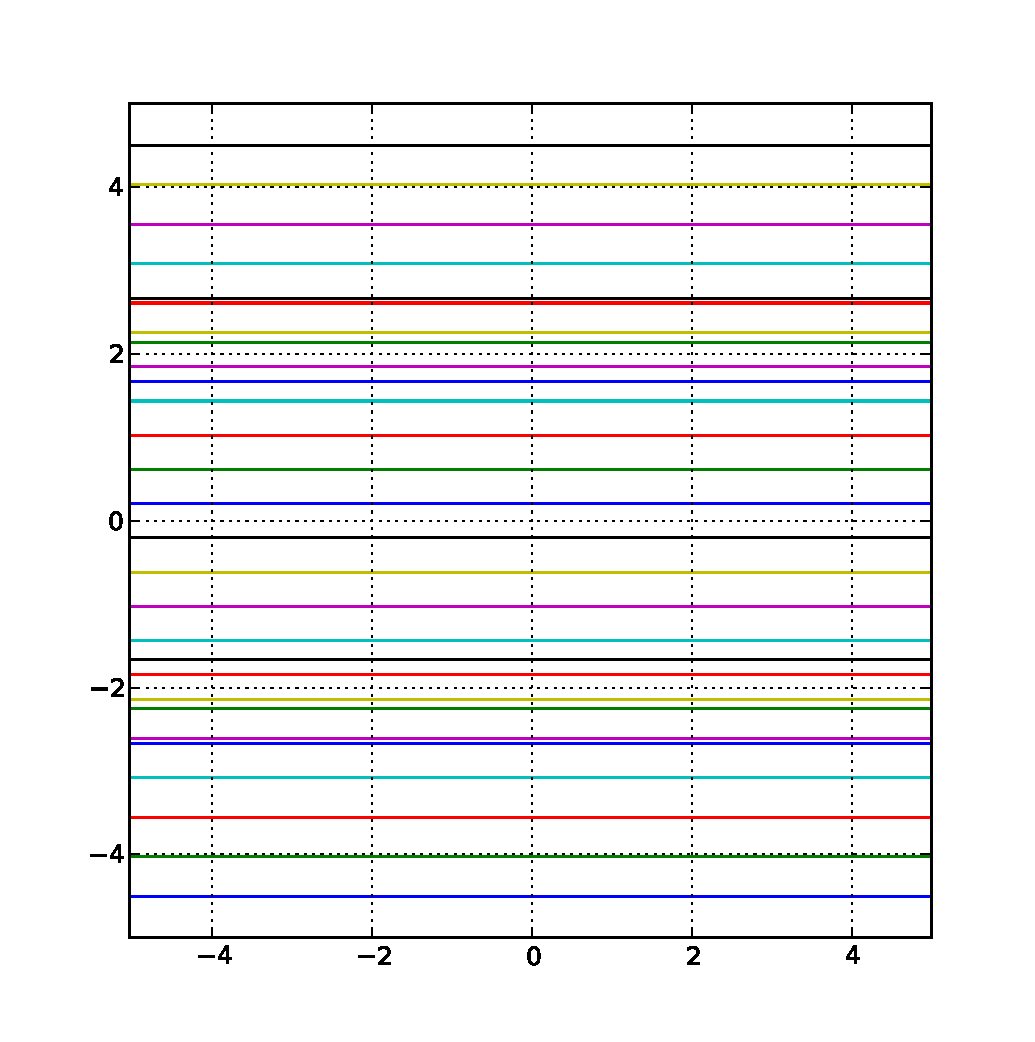
\includegraphics[width=0.45\textwidth]{Images/uniform.pdf}}
%		\subfloat[Source]{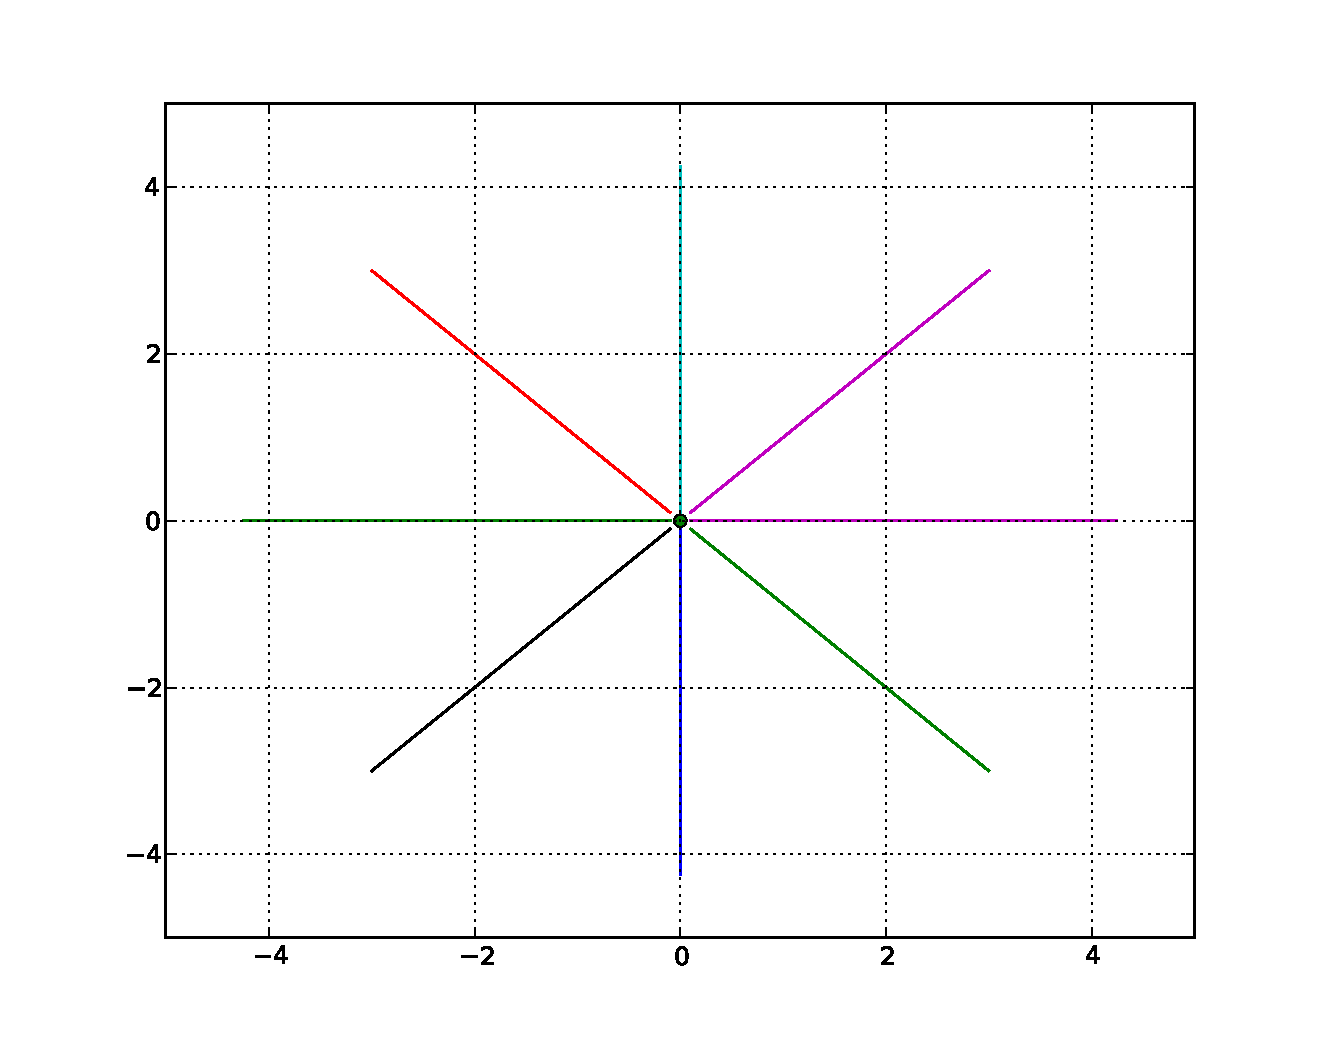
\includegraphics[width=0.45\textwidth]{Images/source.pdf}}
%		\subfloat[Doublet]{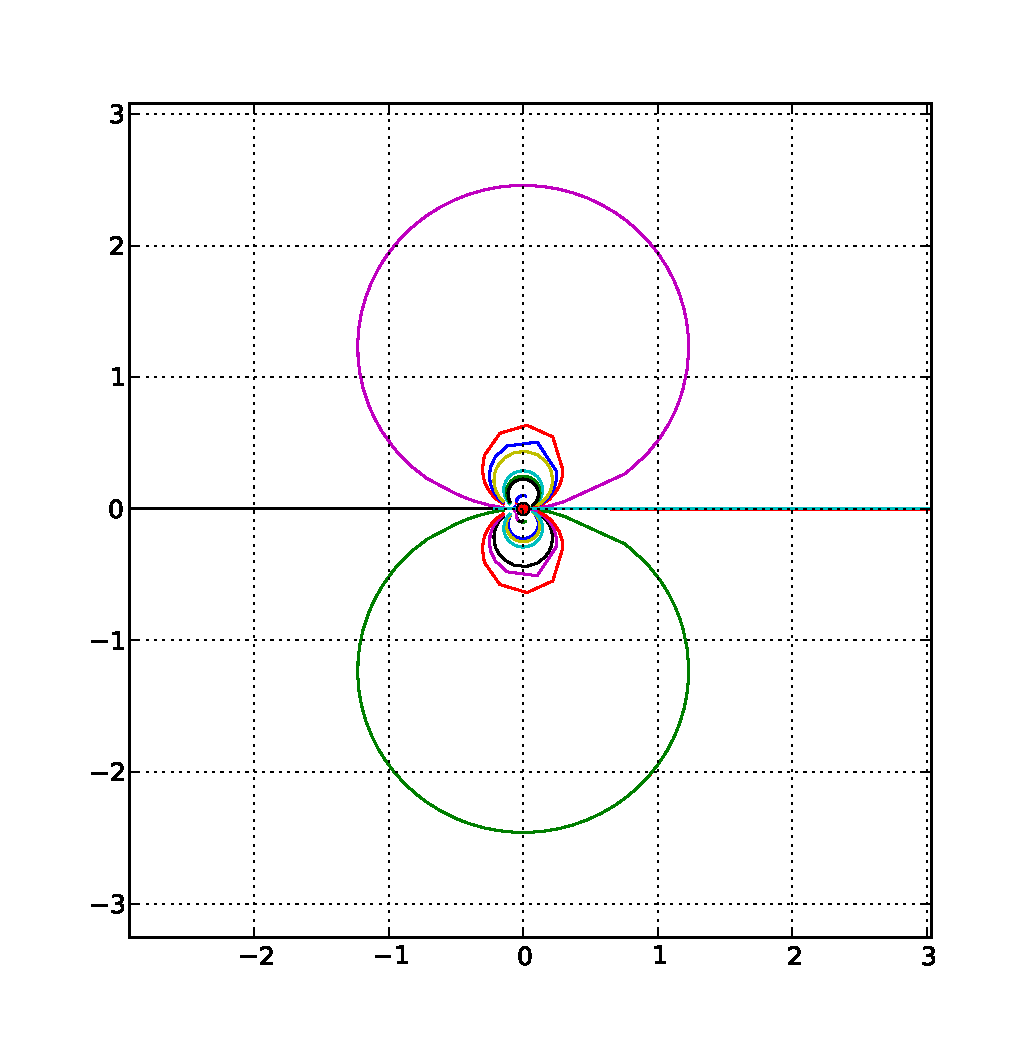
\includegraphics[width=0.45\textwidth]{Images/doublet.pdf}}
%		\subfloat[Vortex]{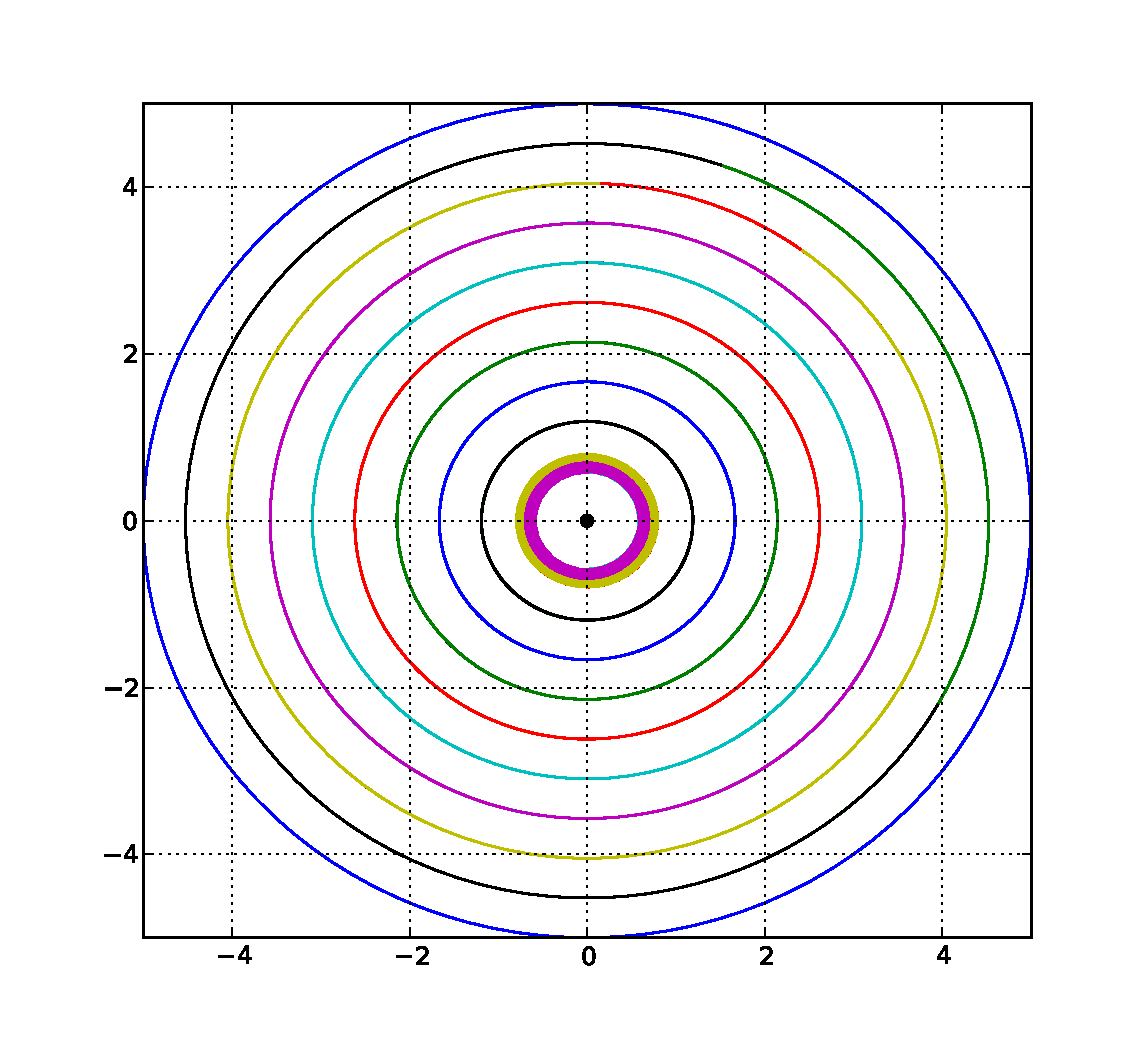
\includegraphics[width=0.45\textwidth]{Images/vortex.pdf}}
%		\caption{Potential flow elements}
%	\end{figure}
%\end{frame}

\section{Potential Flows}
\begin{frame}
	\frametitle{Basic Elements}
	\begin{figure}
		\centering
		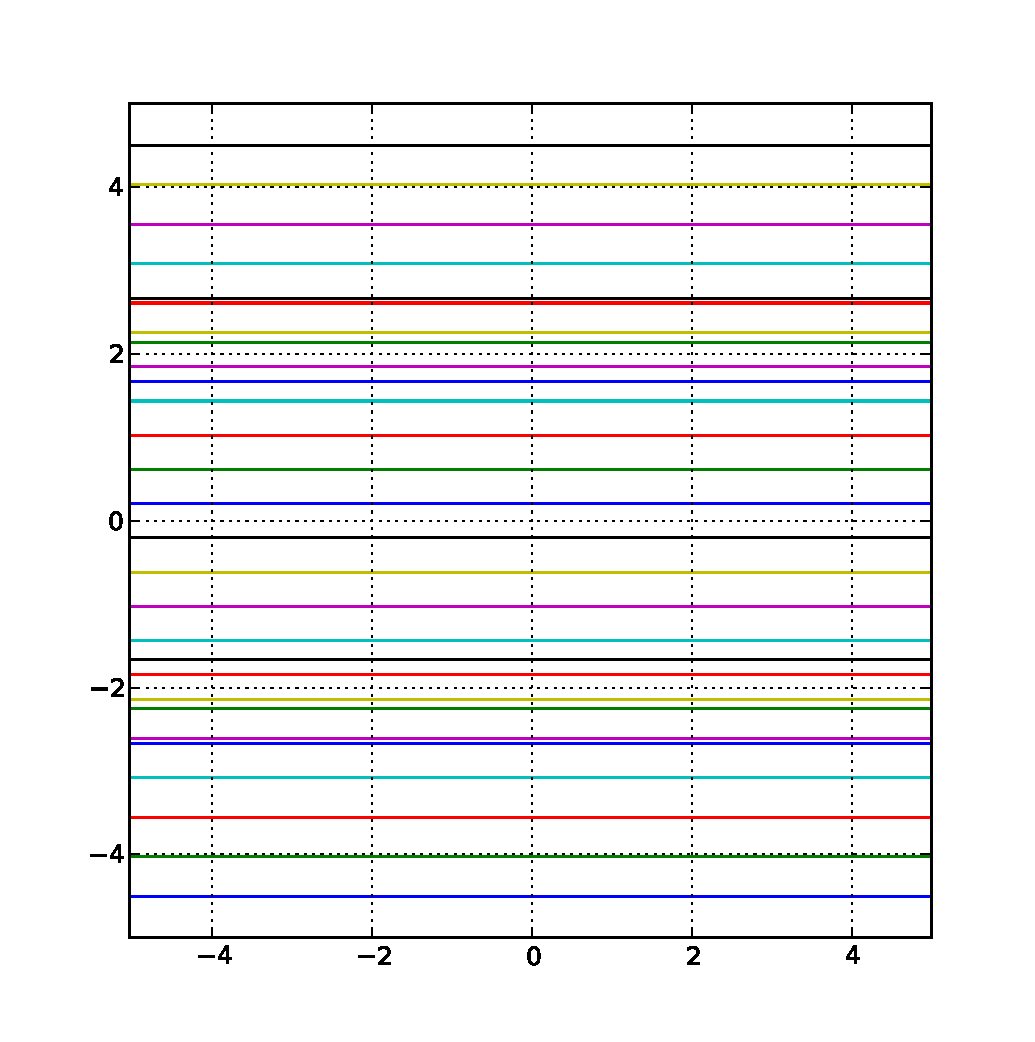
\includegraphics[width=0.3\textwidth]{Images/uniform.pdf}
		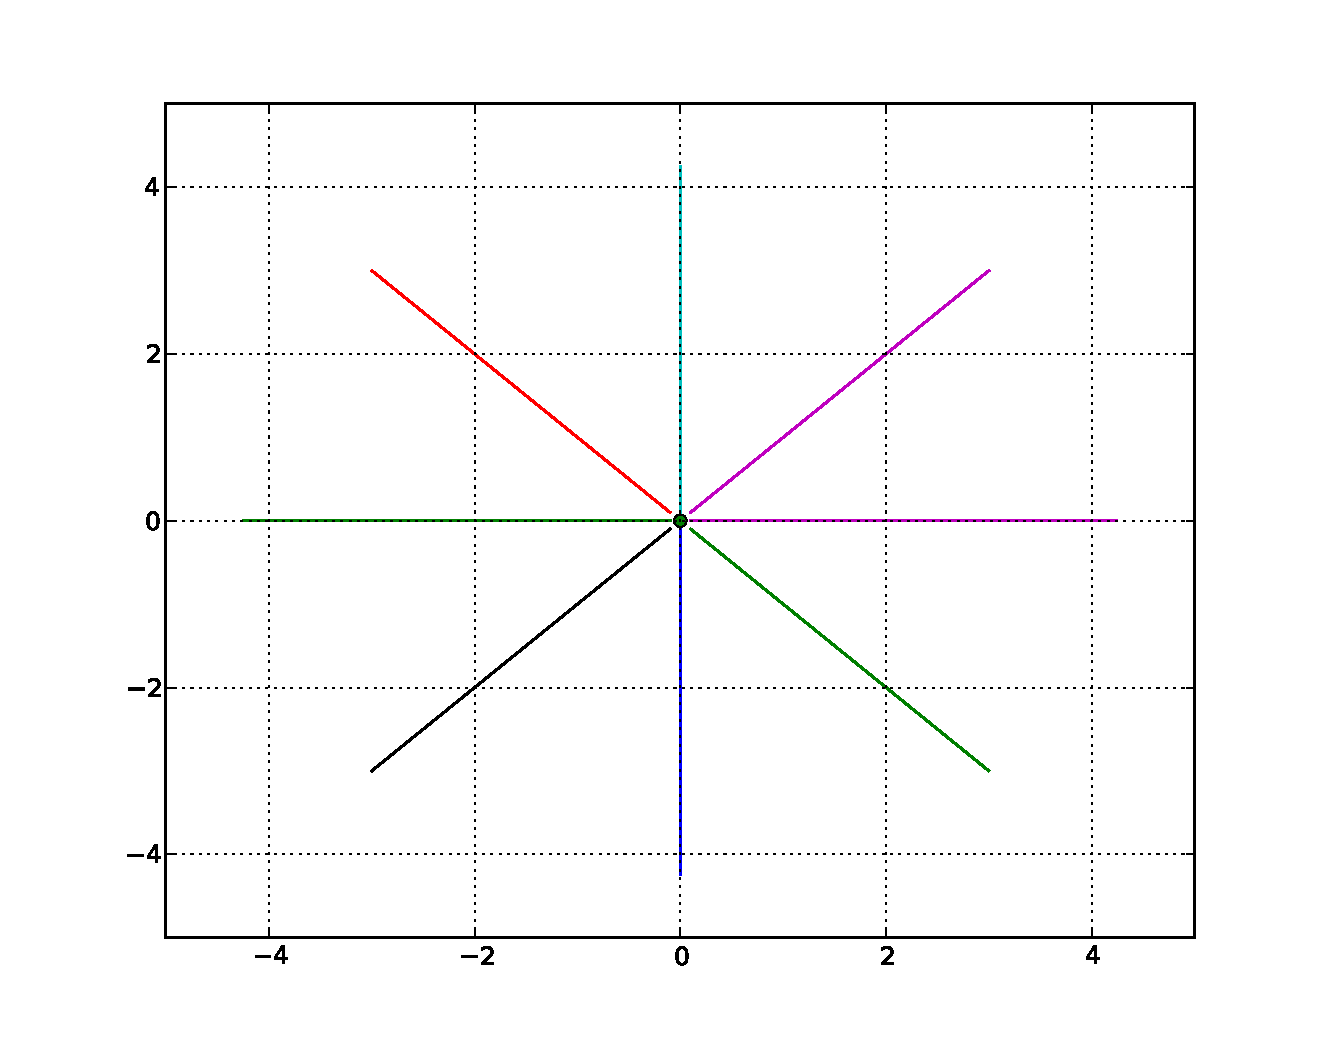
\includegraphics[width=0.3\textwidth]{Images/source.pdf}\\
		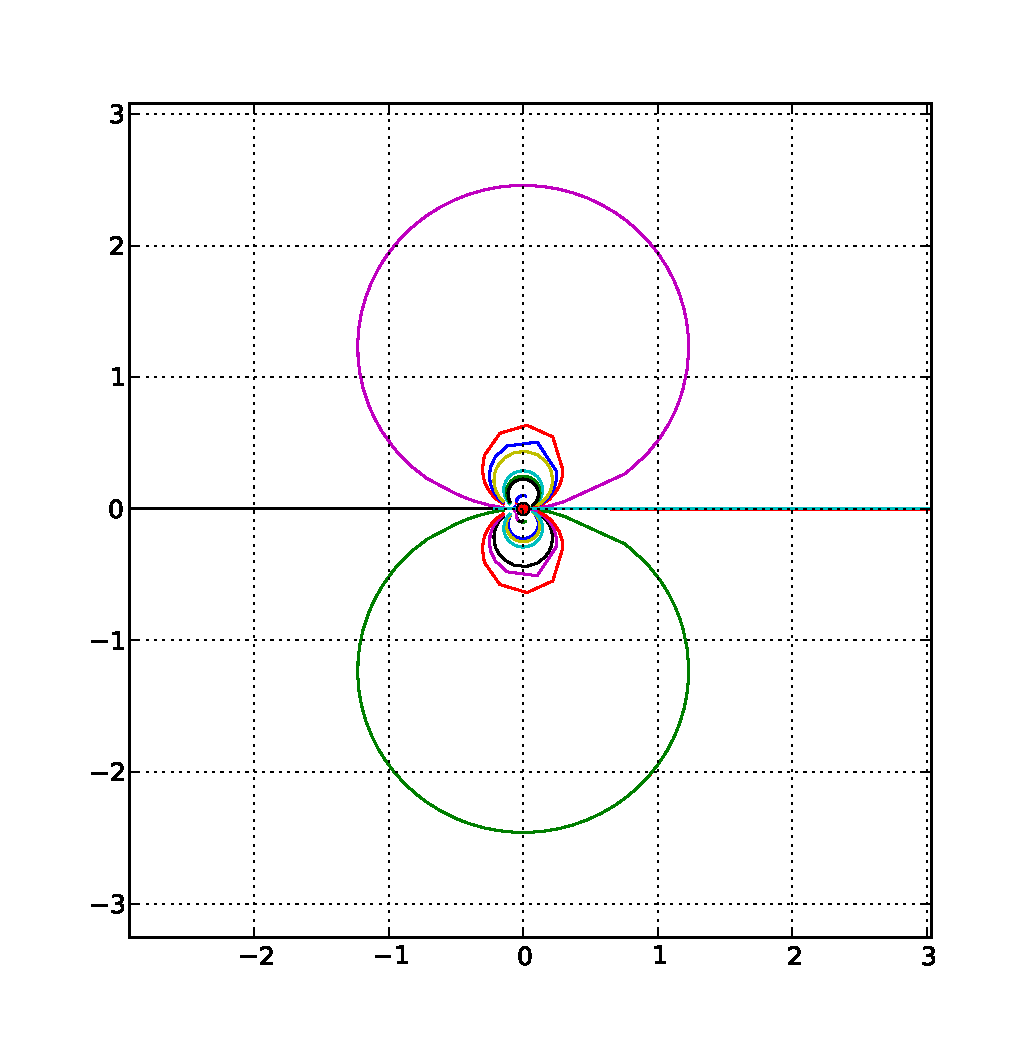
\includegraphics[width=0.4\textwidth]{Images/doublet.pdf}
		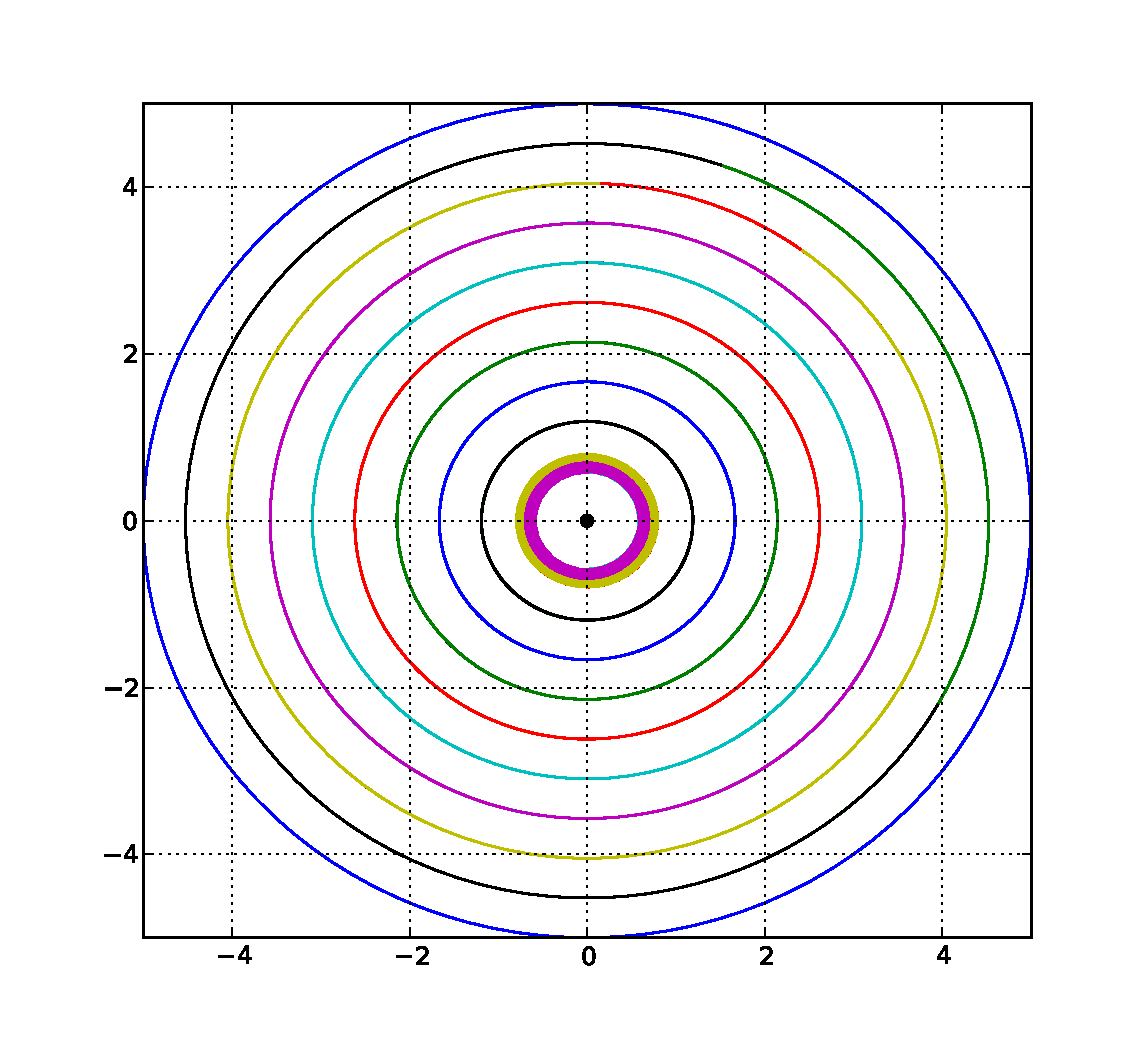
\includegraphics[width=0.4\textwidth]{Images/vortex.pdf}
%		\caption{Uniform Flow, Source}
	\end{figure}
\end{frame}

\begin{frame}
	\frametitle{Basic input features in GUI}
	\begin{itemize}
		\item Add desired potential elements
		\item Interactive plot : \alert{Add} $->$ will be shown in the figure, message in \alert{status bar}
		\item Auto resizing of plotwindow - Not using \alert{auto\_rescale(on)}
			\pause
		\item Can \alert{remove} the elements added!\ldots Also \alert{all} at once!!!
			\pause
		\item \alert{TODO : } Edit the elements added
	\end{itemize}
\end{frame}

\begin{frame}
	\frametitle{Basic output control features in GUI}
	\begin{itemize}
		\item Can plot stream lines - a bit \alert{slow}
	\begin{itemize}
			\item For axis whose length is \alert{10} units, 200$\times$300 values are being considered
			\pause
	\end{itemize}
		\item Tracking evolution of particles - \alert{real time}
			\pause
	\begin{itemize}
			\item Add particles at any desired locations
			\pause
			\item Add patches \begin{enumerate}
				\item At any \alert{X} or \alert{Y} location
				\item Square
				\item Circular
				\end{enumerate}
	\end{itemize}
			\pause
		\item \alert{TODO : } Release particles in rectangular, elliptical, parabolic, hyperbolic patches
	\end{itemize}
\end{frame}

\begin{frame}
	\frametitle{Additional features in GUI}
	\begin{itemize}
		\item Can \alert{play} or \alert{pause} the simulation 
			\pause
		\item Add/Remove elements. Can add new particle during simulation
		\item \alert{Delete} all the particles added for evolution.
			\pause
		\item \alert{Clear plot} without changing the current axis range
			\pause
		\item Can \alert{set} desired \alert{axis limits} for simulation!!!
	\end{itemize}
\end{frame}

\begin{frame}
	\frametitle{Features to be implemented}
	\begin{itemize}
		\item User option to select \alert{blob} to treat the simulation - Currently using \alert{Chorin} blob
			\pause
		\item Velocity, Velocity potential($\phi$) contours
			\pause
		\item Keyboard shortcuts in plot window: \alert{+} for zoom in..etc
			\pause
		\item Continuous potential elements implementation
	\end{itemize}
\end{frame}
\begin{frame}
	\begin{figure}
		\centering
		\includegraphics[width=0.9\textwidth]{Images/network1.png}\\
		\includegraphics[width=0.9\textwidth]{Images/Network0.png}
%		\caption{Uniform Flow, Source}
	\end{figure}
\end{frame}

\begin{frame}
	\begin{center}
		\Huge{Thank you}
	\end{center}
\end{frame}

\end{document}
